\documentclass[runningheads]{llncs}

\usepackage[T1]{fontenc}
\usepackage{graphicx}
\usepackage{amsmath,amssymb}
\usepackage{booktabs}
\usepackage{multirow}
\usepackage{array}
\usepackage{xcolor}
\usepackage{tikz}
\usetikzlibrary{arrows.meta,positioning,fit,calc,backgrounds}
\usepackage{subcaption}
\usepackage[hidelinks]{hyperref}
\usepackage[capitalise,noabbrev]{cleveref}
\usepackage{listings}
\usepackage[section]{placeins}

\renewcommand\UrlFont{\color{blue}\rmfamily}
\lstset{basicstyle=\ttfamily\scriptsize,columns=fullflexible,frame=single,
        framerule=0.3pt,rulecolor=\color{gray},breaklines=true,xleftmargin=2pt}

\makeatletter\newcommand{\tabinput}[1]{\@@input #1 }\makeatother
\newcommand{\R}{\mathbb{R}}
\newcommand{\E}{\mathbb{E}}
\newcommand{\sg}{\operatorname{sg}}
\newcommand{\gp}[1]{\textsc{#1}}

% palette used in every figure (validated categorical slots 1-5)
\definecolor{cNat}{HTML}{2A78D6}
\definecolor{cFsqF}{HTML}{EB6834}
\definecolor{cFsqJ}{HTML}{1BAF7A}
\definecolor{cJep}{HTML}{EDA100}
\definecolor{cGray}{HTML}{8A8A8A}

\begin{document}

\title{Towards a Universal Feature Extractor for Atari Games:\\
Reconstruction, Finite Scalar Quantisation and\\ Joint-Embedding Prediction}
\titlerunning{Towards a Universal Feature Extractor for Atari Games}

\author{Sajid Ali}
\authorrunning{S. Ali}
\institute{TU Dresden, Germany\\[2pt]
Research Project, supervised by Oleh Shkalikov}

\maketitle

\begin{abstract}
Deep reinforcement learning (RL) agents for the Atari 2600 benchmark learn a separate
convolutional feature extractor for every game, even though all games share the same
observation format of four stacked $84\times84$ grey-scale frames. In this project I
investigated whether a \emph{single} visual encoder, pre-trained once on expert
gameplay from eleven games, can serve as a universal feature extractor for Proximal
Policy Optimisation (PPO). I compared three families of self-supervised pre-training
--- pixel reconstruction with a continuous or vector-quantised bottleneck (VAE,
residual VQ-VAE), reconstruction through a Finite Scalar Quantisation (FSQ)
bottleneck, and an action- and environment-conditioned Joint-Embedding Predictive
Architecture (V-JEPA) world model --- and evaluated each encoder either
\emph{frozen} or \emph{jointly fine-tuned} with the policy over 10\,M environment
steps on eleven seen and four held-out games. A jointly fine-tuned FSQ-VAE
matched or exceeded a NatureCNN trained from scratch on 4 of 11 seen games and reached
a higher median human-normalised score (1.07 vs.\ 0.74); on four games it reached 80\%
of the control's final level 1.3--2.7\,M steps earlier. A frozen FSQ encoder retained under
a third of the fine-tuned median (0.31). The V-JEPA encoder, although it learned a
non-collapsed latent space and beat an identity baseline in multi-step latent prediction
on seen games, transferred poorly to control (median HNS 0.05) and did not generalise to
held-out games; neither a pooled 256-dimensional feature nor a stronger entropy bonus
helped. Diagnostics trace this to the objective: the predictor largely ignored the action,
consecutive latents were nearly identical, the latent space was organised by game identity
and specialised to the pre-training games. The results indicate that a shared pre-trained
encoder is a viable \emph{initialisation} but not yet a drop-in \emph{frozen} replacement,
and that a representation useful for control must encode small, fast-moving sprites and
the consequences of actions.

\keywords{Reinforcement learning \and Representation learning \and Atari \and
VQ-VAE \and Finite scalar quantisation \and JEPA \and PPO}
\end{abstract}

% =========================================================================
\section{Introduction}
\label{sec:intro}

Atari 2600 games, exposed through the Arcade Learning Environment
(ALE)~\cite{bellemare2013ale,machado2018revisiting}, are one of the most established
benchmarks for RL from pixels. The canonical pipeline, introduced with
DQN~\cite{mnih2015human} and inherited by policy-gradient methods such as
PPO~\cite{schulman2017ppo}, pre-processes each frame to an $84\times84$ grey-scale image,
stacks the last four frames and feeds the resulting tensor
$x\in[0,1]^{4\times84\times84}$ to a small convolutional network, the \emph{NatureCNN}.
The network's output is consumed by a policy head and/or a value head, and all
components are trained end-to-end from the RL reward alone.

This practice has an obvious inefficiency. Every game is learned from scratch,
including its visual front-end, although all games share the same input format and
much of the same low-level visual vocabulary: sprites, projectiles, walls, scrolling
backgrounds and score digits. A feature extractor that is pre-trained once and reused
across games could (i)~reduce the number of environment interactions needed to learn a
policy, (ii)~reduce computation by removing the need to back-propagate through the
encoder, (iii)~transfer to games it has never seen, and (iv)~provide a common,
inspectable latent space in which different games can be compared.

This project, proposed by Oleh Shkalikov, investigates whether such a
\emph{universal feature extractor} can be trained for Atari. I approached the question
along two axes. The first axis is the \emph{pre-training objective and bottleneck}:
continuous variational autoencoders~\cite{kingma2014vae}, discrete vector-quantised
autoencoders~\cite{vandenoord2017vqvae}, finite scalar
quantisation~\cite{mentzer2024fsq}, and a non-generative, action-conditioned
joint-embedding predictive architecture
(JEPA)~\cite{lecun2022path,assran2023ijepa,bardes2024vjepa}. The second axis is
\emph{where the extractor is trained}: independently of the policy (\emph{frozen}) or
together with it (\emph{joint} fine-tuning from the pre-trained initialisation).

Concretely, the report answers four research questions:
\begin{description}
  \item[RQ1] Which self-supervised objective yields the most useful Atari
  representation for downstream PPO?
  \item[RQ2] Is it better to keep the pre-trained extractor frozen or to fine-tune it
  jointly with the policy and value networks?
  \item[RQ3] Does a representation pre-trained on eleven games generalise to games
  that were never seen during pre-training?
  \item[RQ4] What does the approach cost or save in computation, and does it make
  the learned representation more interpretable?
\end{description}

\paragraph{Contributions.}
\begin{itemize}
  \item Two expert-gameplay corpora covering 15 Atari games: 750\,k frame stacks for
  autoencoders and 2.75\,M transitions $(s_t,a_t,s_{t+1})$ for world-model
  pre-training, with a strict split of 11 pre-training games and 4 held-out games
  (\cref{sec:data}).
  \item A family of interchangeable encoders --- VAE, EMA/residual VQ-VAE with dead-code
  revival, an FSQ-VAE with a resize-convolution decoder and a motion-balanced
  reconstruction loss, and an environment-conditioned V-JEPA with canonical action
  space, SimNorm latents and an inverse-dynamics regulariser (\cref{sec:methods}).
  \item A common PPO integration with frozen and joint modes, and a 10\,M-step
  evaluation on 15 games against a NatureCNN baseline, including an ablation of the
  V-JEPA feature (flattened vs.\ pooled) and of the entropy bonus
  (\cref{sec:setup,sec:results}).
  \item A diagnostic evaluation of the world model that separates genuine latent
  dynamics from two degenerate shortcuts --- representation collapse and copying the
  input frame stack (\cref{sec:jepa-diag}).
\end{itemize}

% =========================================================================
\section{Related Work}
\label{sec:related}

\paragraph{Deep RL on Atari.}
DQN~\cite{mnih2015human} established the NatureCNN encoder and the frame-stacking
convention, and PPO~\cite{schulman2017ppo} with generalised advantage
estimation~\cite{schulman2016gae} became the standard on-policy baseline. Reference
implementations such as Stable-Baselines3~\cite{raffin2021sb3}, its tuned
hyper-parameter zoo~\cite{raffin2020zoo} and CleanRL~\cite{huang2022cleanrl} document
the many details that matter for reproducing PPO on
Atari~\cite{huang2022implementation}. Machado et al.~\cite{machado2018revisiting} and
Agarwal et al.~\cite{agarwal2021precipice} discuss evaluation protocols and the
statistical care needed when comparing agents over few seeds.

\paragraph{Multi-game and generalist agents.}
Training one agent on many Atari games has been approached with distributed
actor--critics (IMPALA~\cite{espeholt2018impala}, PopArt~\cite{hessel2019popart}),
progressive networks~\cite{rusu2016progressive}, and large offline sequence models
such as Multi-Game Decision Transformers~\cite{lee2022multigame} and
Gato~\cite{reed2022gato}. These approaches share the \emph{policy} across games; this
project instead shares only the \emph{perception module} and keeps a per-game policy,
which makes the contribution of the representation measurable in isolation. TD-MPC2~\cite{hansen2024tdmpc2}
conditions a single world model on a learnable per-task embedding; I adopt that
mechanism for the JEPA encoder.

\paragraph{Representation learning for RL.}
Pixel-reconstruction objectives were among the first auxiliary objectives for RL
(World Models~\cite{ha2018worldmodels}, SAC+AE~\cite{yarats2021sac_ae}), and
DARLA~\cite{higgins2017darla} used a $\beta$-VAE~\cite{higgins2017betavae} to obtain
transferable features. DreamerV2~\cite{hafner2021dreamerv2} showed that
\emph{discrete} latents are well suited to Atari, and IRIS~\cite{micheli2023iris}
tokenises frames with a VQ-VAE. Contrastive and self-predictive objectives avoid
reconstruction altogether: CURL~\cite{laskin2020curl}, ATC~\cite{stooke2021atc}, and
SPR~\cite{schwarzer2021spr}, whose pre-training variant SGI~\cite{schwarzer2021sgi}
is the closest precursor to this project's world-model branch. Stooke et
al.~\cite{stooke2021atc} in particular showed that an encoder trained without reward
can be frozen for Atari policy learning in some games. In robotics, pre-trained
visual encoders have been reported both as highly
effective~\cite{parisi2022pvr,nair2022r3m} and as no better than a well-tuned
from-scratch baseline~\cite{hansen2022pretrained}, which is the tension this report
also runs into.

\paragraph{Quantised autoencoders.}
VQ-VAE~\cite{vandenoord2017vqvae} learns a codebook with a straight-through
estimator~\cite{bengio2013ste}; EMA codebook updates~\cite{razavi2019vqvae2} and
reviving unused codes~\cite{dhariwal2020jukebox} are standard remedies for codebook
collapse. Finite Scalar Quantisation (FSQ)~\cite{mentzer2024fsq} replaces the learned
codebook with rounding onto a fixed per-channel integer grid, removing the codebook and
the commitment loss while matching VQ-VAE quality.

\paragraph{Joint-embedding predictive architectures.}
JEPAs predict the representation of a target from the representation of a context,
rather than predicting pixels~\cite{lecun2022path}. I-JEPA~\cite{assran2023ijepa} and
V-JEPA~\cite{bardes2024vjepa} do so for images and video with an EMA target encoder,
following BYOL~\cite{grill2020byol}; why such non-contrastive systems avoid collapse is
analysed in~\cite{chen2021simsiam,tian2021understanding}, and explicit variance
regularisers such as VICReg~\cite{bardes2022vicreg} are an alternative. Inverse-dynamics
objectives, as in ICM~\cite{pathak2017icm}, encourage latents to encode what the agent
controls.

% =========================================================================
\section{Problem Formulation and Background}
\label{sec:background}

\paragraph{Setting.}
Each Atari game $g$ is a partially observable MDP with a game-specific action set
$\mathcal{A}_g\subseteq\{0,\dots,17\}$ ($|\mathcal{A}_g|\in\{4,6,9,14,18\}$ for the
games used here). Following standard pre-processing~\cite{mnih2015human}, the agent
observes $x_t\in\{0,\dots,255\}^{4\times84\times84}$, the last four max-pooled, grey-scale
and down-sampled frames with a frame skip of four. A feature extractor
$f_\theta:\,x\mapsto h\in\R^{d}$ maps the observation to a feature vector on which an
actor $\pi_\omega(a\mid h)$ and a critic $V_\omega(h)$ are trained with
PPO~\cite{schulman2017ppo}, which maximises the clipped surrogate
\begin{equation}
  \mathcal{L}^{\text{CLIP}}(\theta,\omega)=\E_t\big[\min\big(r_t\hat A_t,\;
  \operatorname{clip}(r_t,1-\epsilon,1+\epsilon)\hat A_t\big)\big],\qquad
  r_t=\frac{\pi(a_t\mid x_t)}{\pi_{\text{old}}(a_t\mid x_t)},
\end{equation}
together with a value regression loss and an entropy bonus, using GAE($\lambda$)
advantages $\hat A_t$~\cite{schulman2016gae}.

\paragraph{Universal extractor.}
Let $\mathcal{G}_{\text{pre}}$ be the eleven pre-training games and
$\mathcal{G}_{\text{held}}$ the four held-out games. A universal extractor is a single
set of weights $\theta^\star$, obtained by a self-supervised objective
$\mathcal{L}_{\text{SSL}}$ on data from $\mathcal{G}_{\text{pre}}$ only, that is then
used for PPO on any $g\in\mathcal{G}_{\text{pre}}\cup\mathcal{G}_{\text{held}}$. I
compare three regimes:
\begin{itemize}
  \item \textbf{Scratch (control)}: $\theta$ is randomly initialised and trained by the
  PPO loss (NatureCNN);
  \item \textbf{Frozen}: $\theta=\theta^\star$ is fixed and only $\omega$ is trained;
  \item \textbf{Joint}: $\theta$ is initialised at $\theta^\star$ and trained together
  with $\omega$ by the PPO loss.
\end{itemize}
The frozen regime tests whether the pre-trained representation is \emph{sufficient}
for control; the joint regime tests whether it is a useful \emph{prior}.

% =========================================================================
\section{Data}
\label{sec:data}

Self-supervised pre-training needs frames that resemble what a competent agent sees:
random play rarely leaves the first screen of most games. I therefore collected
gameplay from publicly available pre-trained agents on the HuggingFace Hub (PPO agents
from the RL-Zoo~\cite{raffin2020zoo} where available, otherwise DQN or A2C agents), run
with stochastic action sampling so that the data contains some sub-optimal
behaviour. The environments are \texttt{ALE/*-v5} through Gymnasium~\cite{towers2024gymnasium}
with the Stable-Baselines3 Atari wrapper stack (no-op reset, frame skip 4 with
max-pooling, $84\times84$ grey-scale) and four-frame stacking.

\begin{table}[t]
\centering
\caption{Game split and data sources. Expert agents are downloaded from the
HuggingFace Hub. $|\mathcal{A}_g|$ is the size of each game's minimal action set.}
\label{tab:games}
\footnotesize\setlength{\tabcolsep}{4pt}
\begin{tabular}{@{}llcl@{}}
\toprule
Split & Games & $|\mathcal{A}_g|$ & Expert \\
\midrule
\multirow{4}{*}{Pre-training (11)}
 & Breakout & 4 & PPO \\
 & Pong, Qbert, SpaceInv., DemonAttack & 6 & PPO (DemonAtt.: DQN) \\
 & BeamRider, Enduro, MsPacman & 9 & PPO \\
 & Riverraid, Seaquest, RoadRunner & 18 & PPO (RoadRunner: A2C) \\
\midrule
\multirow{2}{*}{Held-out (4)}
 & Atlantis & 4 & DQN \\
 & Asteroids / Alien, IceHockey & 14 / 18 & DQN \\
\bottomrule
\end{tabular}
\end{table}

Two corpora were built (\cref{tab:games,tab:corpora,fig:data}):
\begin{enumerate}
  \item \textbf{Frame corpus} for the autoencoders: 50\,000 consecutive frame stacks per
  game, i.e.\ 550\,k stacks from the pre-training games and 200\,k from the held-out
  games, stored as \texttt{uint8} arrays of shape $(N,84,84,4)$.
  \item \textbf{Transition corpus} for the world model: tuples
  $(s_t,a_t,s_{t+1},\text{terminal}_t)$ with 250\,000 transitions per pre-training game
  (2.75\,M in total, stored in five compressed shards per game), a validation split of
  10\,000 transitions per pre-training game collected with a different seed, and
  50\,000 transitions per held-out game. At episode ends the true terminal observation is
  stored instead of the auto-reset observation.
\end{enumerate}

\begin{table}[t]
\centering
\caption{Datasets used in this project.}
\label{tab:corpora}
\setlength{\tabcolsep}{5pt}
\begin{tabular}{@{}lrrl@{}}
\toprule
Corpus & Games & Samples & Used by \\
\midrule
Frame stacks (train) & 11 & 550\,k & VAE / VQ-VAE / FSQ-VAE \\
Frame stacks (test) & 4 held-out & 200\,k & reconstruction test loss \\
Transitions (train) & 11 & 2.75\,M & V-JEPA pre-training \\
Transitions (val) & 11 & 110\,k & V-JEPA model selection \\
Transitions (test) & 4 held-out & 200\,k & zero-shot diagnostics \\
\bottomrule
\end{tabular}
\end{table}

\begin{figure}[t]
\centering
\input{figures/data_pipeline}
\caption{(a)~Data collection: pre-trained expert agents play each game through the
standard Atari pre-processing, with actions sampled from their policies; the resulting
frame stacks and transitions form the two corpora. (b)~Processing applied when training
on them: consecutive stacks share three frames, transitions that end an episode are
masked out of the loss, game-specific action indices are mapped to the canonical ALE-18
set, and the FSQ-VAE loss up-weights pixels that move within a stack.}
\label{fig:data}
\end{figure}

Two properties of this data shaped the later design. First, \emph{consecutive frame
stacks overlap}: $s_{t+1}$ contains three of the four frames of $s_t$, and I measured
that \texttt{next\_obs[...,:3] == obs[...,1:]} holds for 100\% of the stored
transitions. A one-step prediction target is therefore 75\% identical to the input.
Second, the stored actions index each game's \emph{minimal} action set, so the same
integer means different joystick commands in different games (index 3 is
\textsc{Left} in Breakout but \textsc{Right} in Seaquest). \Cref{sec:jepa} describes how
both were handled. Sticky actions~\cite{machado2018revisiting} were disabled during
collection.

% =========================================================================
\section{Methods}
\label{sec:methods}

\Cref{fig:overview} summarises the pipeline. All encoders consume
$x\in[0,1]^{4\times84\times84}$ and differ in their pre-training objective, their
bottleneck, and the feature vector they hand to PPO (\cref{tab:encoders}).

\begin{figure}[t]
\centering
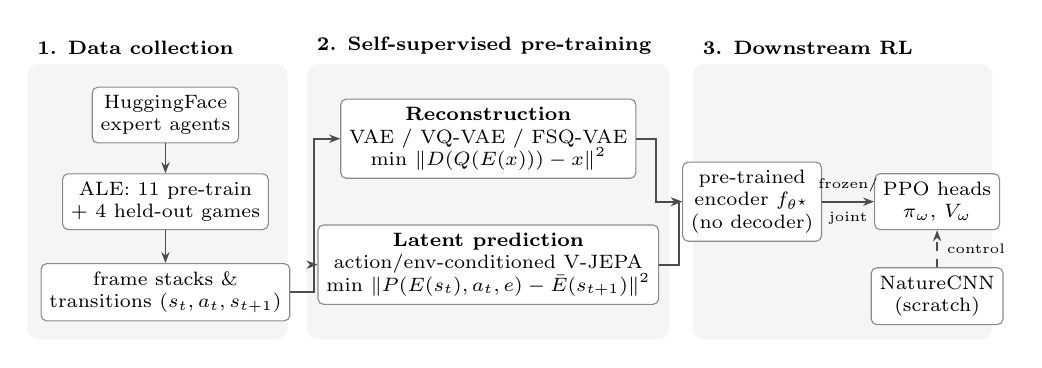
\begin{tikzpicture}[
  font=\scriptsize,
  box/.style={draw=cGray, rounded corners=2pt, align=center, inner sep=3pt, fill=white},
  lab/.style={font=\scriptsize\bfseries, anchor=south west},
  arr/.style={-{Stealth[length=4pt]}, draw=black!70, line width=0.6pt}]
  \fill[gray!8, rounded corners=4pt] (-0.25,0) rectangle (3.05,3.5);
  \fill[gray!8, rounded corners=4pt] (3.3,0) rectangle (7.9,3.5);
  \fill[gray!8, rounded corners=4pt] (8.2,0) rectangle (12.0,3.5);
  \node[lab] at (-0.25,3.5) {1. Data collection};
  \node[lab] at (3.3,3.5) {2. Self-supervised pre-training};
  \node[lab] at (8.2,3.5) {3. Downstream RL};
  \node[box] (hub) at (1.5,2.85) {HuggingFace\\expert agents};
  \node[box] (env) at (1.5,1.75) {ALE: 11 pre-train\\+ 4 held-out games};
  \node[box] (data) at (1.5,0.6) {frame stacks \&\\transitions $(s_t,a_t,s_{t+1})$};
  \draw[arr] (hub) -- (env); \draw[arr] (env) -- (data);
  \node[box] (rec) at (5.6,2.55) {\textbf{Reconstruction}\\VAE / VQ-VAE / FSQ-VAE\\$\min\,\|D(Q(E(x)))-x\|^2$};
  \node[box] (jep) at (5.6,0.95) {\textbf{Latent prediction}\\action/env-conditioned V-JEPA\\$\min\,\|P(E(s_t),a_t,e)-\bar E(s_{t+1})\|^2$};
  \draw[arr] (data.east) -- ++(0.3,0) |- (rec.west);
  \draw[arr] (data.east) -- ++(0.3,0) |- (jep.west);
  \node[box] (enc) at (8.95,1.75) {pre-trained\\encoder $f_{\theta^\star}$\\(no decoder)};
  \node[box] (ppo) at (11.3,1.75) {PPO heads\\$\pi_\omega,\,V_\omega$};
  \node[box] (cnn) at (11.3,0.55) {NatureCNN\\(scratch)};
  \draw[arr] (rec.east) -- ++(0.25,0) |- (enc.west);
  \draw[arr] (jep.east) -- ++(0.25,0) |- (enc.west);
  \draw[arr] (enc) -- node[above, font=\tiny]{frozen/} node[below, font=\tiny]{joint} (ppo);
  \draw[arr, dashed] (cnn) -- node[right, font=\tiny]{control} (ppo);
\end{tikzpicture}
\caption{Overview of the three stages. One encoder is pre-trained on the eleven
pre-training games and reused for PPO on every game, either frozen or jointly
fine-tuned. A NatureCNN trained from scratch per game is the control.}
\label{fig:overview}
\end{figure}

\begin{table}[t]
\centering
\caption{Encoders studied. ``Feature'' is the vector passed to the PPO heads.}
\label{tab:encoders}
\footnotesize\setlength{\tabcolsep}{3pt}
\begin{tabular}{@{}lllll@{}}
\toprule
Encoder & Backbone & Bottleneck & Latent grid & Feature \\
\midrule
NatureCNN~\cite{mnih2015human} & 3 conv + FC & none & $64\times7\times7$ & 512 \\
VAE & NatureCNN conv & Gaussian, $d=256$ & -- & 256 ($\mu$) \\
Residual VQ-VAE & conv + 2 res.\ blocks & VQ, $K=512$, $d=64$ & $64\times21\times21$ & 28\,224 \\
FSQ-VAE & 3 conv & FSQ $L=[8,5,5,3]$ & $4\times21\times21$ & 1\,764 \\
V-JEPA & ViT, 6 layers & SimNorm, $V=8$ & $36\times256$ tokens & 9\,216 \\
\bottomrule
\end{tabular}
\end{table}

% -------------------------------------------------------------------------
\subsection{Continuous VAE}
\label{sec:vae}

The first baseline is a Gaussian VAE~\cite{kingma2014vae} whose encoder is exactly the
NatureCNN convolutional trunk ($32@8{\times}8/4 \rightarrow 64@4{\times}4/2 \rightarrow
64@3{\times}3/1$, giving $64\times7\times7=3136$ units), followed by linear heads for
$\mu,\log\sigma^2\in\R^{256}$. A mirrored transposed-convolution decoder with a sigmoid
output reconstructs the frame stack, and the model minimises
$\mathcal{L}_{\text{VAE}}=\|\hat x-x\|_2^2+\beta\,D_{\text{KL}}\big(q(z\mid x)\,\|\,\mathcal{N}(0,I)\big)$.
The motivation is that the encoder is architecturally identical to the RL baseline, so any
difference can be attributed to the objective. In practice, reconstruction-trained
continuous autoencoders on Atari are known to blur small objects and, with a strong KL
term, to ignore parts of the input (posterior
collapse~\cite{bowman2016posterior}); compressing $84\times84$ to a $7\times7$ grid
additionally leaves each latent cell responsible for a $12\times12$ pixel region, far larger
than a Pong ball or a Space Invaders bullet. For these reasons the VAE was trained only
for a single exploratory epoch (the only VAE run in the experiment log), was not carried
forward to the 10\,M-step RL evaluation, and the project moved to spatial, discrete
bottlenecks.

% -------------------------------------------------------------------------
\subsection{Vector-Quantised VAE with EMA Codebook}
\label{sec:vqvae}

The residual VQ-VAE keeps a spatial latent grid at $21\times21$ (four times finer than
NatureCNN) by using two stride-2 convolutions ($84\to42\to21$), a $3\times3$ convolution,
and a stack of two residual blocks~\cite{he2016resnet}, followed by a $1\times1$
projection to $d=64$ channels. Each of the $441$ latent vectors $z_e$ is replaced by its
nearest codeword $e_k$ in a codebook of $K=512$ entries,
\begin{equation}
  z_q = e_{k^\star},\quad k^\star=\arg\min_k \|z_e-e_k\|_2,\qquad
  \tilde z_q = z_e + \sg(z_q - z_e),
\end{equation}
where the straight-through estimator $\tilde z_q$~\cite{bengio2013ste} passes decoder
gradients to the encoder. The codebook is not trained by gradient descent but by
exponential moving averages of cluster sizes and assigned vectors (decay $\gamma=0.99$,
following~\cite{vandenoord2017vqvae,razavi2019vqvae2}), and the encoder is pulled towards
its codes by a commitment loss $\beta\|z_e-\sg(z_q)\|^2$ with $\beta=0.25$. To prevent
codebook collapse, any code whose EMA usage falls below one is re-initialised to a
random encoder output from the current batch (\emph{dead-code
revival}~\cite{dhariwal2020jukebox}).

\paragraph{Sprite-weighted loss.}
In Atari frames almost all pixels are static background, so a plain MSE is dominated by
the background and the decoder can drop small moving objects at almost no cost. I
therefore computed a motion mask from the frame stack itself,
$m=\mathbb{1}\big[\max_{j}|x^{(j+1)}-x^{(j)}|>\delta\big]$, and up-weighted moving
pixels by a factor of ten. As \cref{sec:recon} shows, this trades background fidelity
for sprite fidelity: with a fixed code budget, the codebook moves capacity towards
sprites and away from static elements such as score digits.

% -------------------------------------------------------------------------
\subsection{FSQ-VAE with Resize-Convolution Decoder}
\label{sec:fsq}

Finite Scalar Quantisation~\cite{mentzer2024fsq} removes the codebook altogether. The
encoder (two stride-2 convolutions and one $3\times3$ convolution, 128 channels) is
projected by a $1\times1$ convolution to $C=4$ channels, and each channel $c$ is
quantised independently onto $L_c$ levels:
\begin{equation}
  u=\sigma(z_e),\qquad
  z_q = \frac{2\,\operatorname{round}\big(u\,(L_c-1)\big)}{L_c-1}-1,\qquad
  \tilde z_q = (2u-1) + \sg\big(z_q-(2u-1)\big).
\end{equation}
With $L=[8,5,5,3]$ every latent cell takes one of $8\cdot5\cdot5\cdot3=600$ values, an
implicit codebook of the same order as the VQ-VAE's, but with no distance computation,
no EMA statistics, no commitment loss and no possibility of dead codes. Using a sigmoid
rather than the $\tanh$ with half-integer offsets of the original paper keeps the grid
exact for even level counts ($L_1=8$); an earlier $\tanh$ variant I implemented could only reach
7 of the 8 levels for $L_1=8$.

\paragraph{Decoder and loss.}
The first FSQ-VAE used transposed convolutions and showed checkerboard
artefacts~\cite{odena2016deconvolution}, which are particularly harmful on flat Atari
backgrounds. The final decoder therefore uses \emph{resize-convolutions}: two
$3\times3$ convolutions at $21\times21$, nearest-neighbour up-sampling to $42\times42$,
two convolutions, up-sampling to $84\times84$, and two convolutions with a sigmoid
output. Instead of the multiplicative sprite weight of \cref{sec:vqvae}, the loss
normalises the moving and static regions separately and then mixes them with a fixed
ratio,
\begin{equation}
  \mathcal{L}_{\text{bal}} = w\,\frac{\sum m\odot(\hat x-x)^2}{\sum m}
  +(1-w)\,\frac{\sum (1-m)\odot(\hat x-x)^2}{\sum (1-m)},\qquad w=0.85,\;\delta=0.05,
\end{equation}
so that moving pixels receive a fixed 85\% of the gradient regardless of how few of them
there are, while the background is still reconstructed. When a stack contains no motion
(or only motion) the loss falls back to the plain MSE.

For PPO, the decoder is discarded and the quantised grid $\tilde z_q\in[-1,1]^{4\times21\times21}$
is flattened into a 1\,764-dimensional feature vector.

% -------------------------------------------------------------------------
\subsection{Action- and Environment-Conditioned V-JEPA}
\label{sec:jepa}

Reconstruction forces an encoder to spend capacity on every pixel, including those that
are irrelevant for control. A JEPA instead learns to \emph{predict the representation of
the next observation}~\cite{lecun2022path}. Conditioning the prediction on the action
turns it into a latent world model, in the spirit of SPR~\cite{schwarzer2021spr} and
SGI~\cite{schwarzer2021sgi}. \Cref{fig:jepa} shows the final (v2) architecture.

\begin{figure}[t]
\centering
\input{figures/jepa_arch}
\caption{Environment- and action-conditioned V-JEPA (v2), as implemented. The context
encoder, predictor, game and action embeddings and the inverse head are trained; the
target encoder is an EMA copy of the context encoder whose outputs are the regression
targets. The game embedding is a token in both encoders and the predictor, and is
replaced by UNKNOWN with probability 0.25. Only the context encoder is kept for PPO.}
\label{fig:jepa}
\end{figure}

\paragraph{Encoders.}
A $14\times14$ patch embedding turns the four-frame stack into a $6\times6=36$-token
sequence of width $D=256$ with learned positional embeddings~\cite{dosovitskiy2021vit}.
The context encoder $E_\theta$ is a six-layer pre-LayerNorm~\cite{xiong2020prenorm}
transformer~\cite{vaswani2017attention} with eight heads and GELU MLPs. The target
encoder $\bar E$ is an exponential moving average of $E_\theta$,
$\bar\theta\leftarrow\tau\bar\theta+(1-\tau)\theta$ with $\tau=0.996$, and receives no
gradients, as in BYOL and I-JEPA~\cite{grill2020byol,assran2023ijepa}.

\paragraph{Predictor.}
The predictor $P_\psi$ is a shallower three-layer transformer that receives the 36
context tokens, prepended with a learned action token $a_t$ and an environment token
(below), and outputs 36 predicted target tokens. The training objective is the masked
latent regression
\begin{equation}
  \mathcal{L}_{\text{JEPA}}=\frac{\sum_i m_i\,\big\|P_\psi\big(E_\theta(s_t^i,e^i),a_t^i,e^i\big)
  -\sg\big(\bar E(s_{t+1}^i,e^i)\big)\big\|_2^2}{\sum_i m_i},
\end{equation}
where $m_i=0$ at episode ends so that no loss is computed across episode boundaries.

\paragraph{From v1 to v2.}
The first version (v1) trained well by its loss curve, but a systematic audit of the
pipeline revealed problems that made its action conditioning incoherent. Its two
100-epoch production runs also never completed: they ended after exactly 4\,h and 8\,h
of wall-clock time, i.e.\ at the job time limit, after 10 and 19 epochs. Following that
audit I re-designed the model (v2), largely along the lines of
TD-MPC2~\cite{hansen2024tdmpc2}:
\begin{enumerate}
  \item \textbf{Canonical action space.} Stored minimal-set action indices are
  mapped through a per-game look-up table to the canonical 18-action ALE enumeration, so
  the shared action embedding means the same joystick command in every game.
  \item \textbf{Environment embedding.} A learnable embedding $e_g\in\R^{256}$,
  $\|e_g\|\le1$, per game is prepended as a token to both encoders and to the
  predictor, so the same visual pattern can be interpreted differently in different
  games. The table has 16 rows: 11 pre-training games, one UNKNOWN slot and four
  pre-allocated rows for the held-out games.
  \item \textbf{Environment dropout.} With probability 0.25 the game identity is replaced
  by UNKNOWN (as in classifier-free guidance~\cite{ho2021cfg}). This trains a generic
  ``Atari prior'' that can be used zero-shot on unseen games and discourages the encoder
  from splitting into eleven disjoint sub-spaces.
  \item \textbf{SimNorm.} All three latents are projected onto a product of 32 simplices
  of size $V=8$ (TD-MPC2, Eq.~5),
  \[\operatorname{SimNorm}(z)=\big[\operatorname{softmax}(z_{1:8}),\dots,\operatorname{softmax}(z_{249:256})\big],\]
  which bounds the latent and removes the \emph{scale} route to representation collapse.
  \item \textbf{Inverse-dynamics regulariser.} An MLP predicts $a_t$ from the mean-pooled
  latents of $s_t$ and $s_{t+1}$ and the environment embedding, with logits masked to the
  game's valid actions. The total loss is $\mathcal{L}=\mathcal{L}_{\text{JEPA}}+\lambda\,\mathcal{L}_{\text{inv}}$.
  Because SimNorm shrinks $\mathcal{L}_{\text{JEPA}}$ by an order of magnitude
  (0.026 at initialisation vs.\ $\approx$2.2\,nats for $\mathcal{L}_{\text{inv}}$), $\lambda$
  was reduced from 0.1 to 0.01, and a sweep over $\{0.003,0.01,0.03,0.1\}$ was run to
  confirm the choice (\cref{sec:pretrain-res}).
  \item \textbf{Instrumentation.} Per-game losses, representation-health statistics
  (per-dimension standard deviation and effective rank~\cite{roy2007effective}) with an
  untrained reference, the information gain of the inverse head relative to its chance
  floor $\log|\mathcal{A}_g|$, and the geometry of the game embeddings.
\end{enumerate}
The audit also found and fixed data-pipeline bugs: an unconditional HWC$\to$CHW transpose
that made the full 2.75\,M-transition corpus unusable by v1 (it was stored CHW), and a
validation sampler that silently evaluated only the first game's shard.

\paragraph{Feature for PPO.}
The frozen or fine-tuned context encoder, conditioned on the game's own embedding (or
UNKNOWN for unseen games), produces $36\times256$ SimNorm tokens. In the main runs
these are flattened into a 9\,216-dimensional feature vector. A second set of runs
pools the 36 tokens into a single 256-dimensional vector (no added parameters) and gives
the actor and the critic separate copies of the extractor (\cref{sec:rl}).

% =========================================================================
\section{Experimental Setup}
\label{sec:setup}

\paragraph{Training configurations.}
\Cref{tab:pretrain} lists the configuration of every encoder that was carried to PPO,
next to the setting of the paper each design follows. The FSQ-VAE was trained for 125
epochs on the 550\,k-stack frame corpus with AdamW~\cite{loshchilov2019adamw}, a constant
learning rate for 100 epochs followed by cosine decay~\cite{loshchilov2017sgdr}, bf16
autocast and \texttt{torch.compile}. The residual VQ-VAEs (plain and sprite-weighted) were
trained for 15 epochs on Google Colab. The V-JEPA v2 model was trained on one NVIDIA H100
on the TU Dresden HPC cluster, with a throughput probe that sized the cosine schedule to
the wall-clock allocation. It ran for 92 epochs ($\approx$10.9\,M samples or 3.9 passes
over the corpus), and the checkpoint with the lowest validation loss (epoch 90) was used.
The NatureCNN control has no pre-training: it is trained by PPO alone, with the
hyper-parameters of \cref{tab:ppo}. The continuous VAE, which was not carried to PPO, was
trained for one epoch (batch 64, Adam, $10^{-4}$), against minibatches of 100 with Adagrad
in the original work~\cite{kingma2014vae}. All runs were logged to Weights \&
Biases~\cite{biewald2020wandb}, and every number in \cref{sec:results} is computed from
the full, unsampled logged histories.

\paragraph{Relation to the reference settings.}
The architectural choices follow the references closely: the VQ-VAE uses the original
codebook size ($K=512$), commitment weight ($\beta=0.25$) and EMA decay ($\gamma=0.99$);
the V-JEPA uses the I-JEPA patch size of 14, AdamW with warm-up and cosine decay, and an
EMA target with the I-JEPA starting momentum of 0.996; SimNorm uses TD-MPC2's $V=8$ and
its game embedding TD-MPC2's norm bound of 1; and the NatureCNN agent uses the Atari PPO
setting of Schulman et al.\ as packaged by the RL-Zoo. The deviations are deliberate and
driven by scale. The JEPA references train ViT-H models for 90\,k--300\,k large-batch
iterations on millions of natural images or videos. A 12.5\,M-parameter model on
$84\times84$ Atari frames on one GPU called for a smaller batch (512 instead of
2\,048--3\,072), a lower peak learning rate ($3\cdot10^{-4}$, the TD-MPC2 value, instead
of $10^{-3}$ or $6.25\cdot10^{-4}$) and a much smaller weight decay than the 0.04--0.4
schedule. The EMA momentum was kept fixed at 0.996; the momentum schedule towards 1.0
used by I-JEPA and V-JEPA was not implemented. The FSQ level set $[8,5,5,3]$ (600 codes)
lies between the paper's recommendations for $2^8$ and $2^{10}$ codes. The PPO runs use
the RL-Zoo variant of the paper's setting (four instead of three epochs, value coefficient
0.5 instead of 1), which is the standard for Stable-Baselines3.

\begin{table}[t]
\centering
\caption{Training configurations of the four encoders used with PPO (``this work'') and
the setting of the reference paper each follows. ``--'': not specified, or not logged.}
\label{tab:pretrain}
\scriptsize\setlength{\tabcolsep}{2.5pt}
\newcolumntype{Y}[1]{>{\raggedright\arraybackslash}p{#1}}
\begin{tabular}{@{}Y{1.6cm}Y{2.25cm}Y{2.2cm}Y{2.95cm}Y{2.25cm}@{}}
\toprule
 & Residual VQ-VAE & FSQ-VAE & V-JEPA v2 & NatureCNN \\
\midrule
\multicolumn{5}{@{}l}{\textit{This work}} \\
Objective & MSE$^{a}$ + VQ + commit. & $\mathcal{L}_{\text{bal}}$, $w=0.85$ &
  $\mathcal{L}_{\text{JEPA}}+0.01\,\mathcal{L}_{\text{inv}}$ & PPO only (no pre-training) \\
Data & 550\,k stacks & 550\,k stacks & 2.75\,M transitions & online, $10^7$ steps/game \\
Length & 15 ep.\ (129\,k steps) & 125 ep.\ (537\,k steps) & 92 ep.\ (21.2\,k steps) & 9.8\,k rollouts \\
Batch & 64 & 128 & 512 & $8\times128$; minibatch 256 \\
Optimiser, LR & $3{\cdot}10^{-4}$ & AdamW, $3{\cdot}10^{-4}$ & AdamW, $3{\cdot}10^{-4}$ & Adam, $2.5{\cdot}10^{-4}\to0$ \\
Weight decay & -- & $10^{-4}$ & $10^{-5}$ (not LN/emb.) & 0 \\
Schedule & -- & 100 ep.\ const.\ + cosine & warm-up + cosine & linear to 0 \\
Bottleneck / target & $K{=}512$, $d{=}64$, $\beta{=}0.25$, EMA 0.99 & FSQ $L{=}[8,5,5,3]$ (600) &
  EMA $\tau{=}0.996$ (fixed); SimNorm $V{=}8$; patch 14 & -- \\
Parameters & 0.70\,M & 0.84\,M & 12.5\,M & 1.68\,M \\
Hardware, time & Tesla T4, 3.0\,h & H100, 1.9\,h & H100, 15.6\,h & H100, 3.0\,h/game \\
\midrule
\multicolumn{5}{@{}l}{\textit{Reference setting}} \\
Source & VQ-VAE~\cite{vandenoord2017vqvae} & FSQ~\cite{mentzer2024fsq} &
  I-JEPA~\cite{assran2023ijepa} / V-JEPA~\cite{bardes2024vjepa} / TD-MPC2~\cite{hansen2024tdmpc2} &
  PPO~\cite{schulman2017ppo}, RL-Zoo~\cite{raffin2020zoo} \\
Length & 250\,k steps & -- & 300 ep.\ / 90\,k it. / -- & $10^7$ steps (40\,M frames) \\
Batch & 128 & -- & 2\,048 / 3\,072 / 256 & $8\times128$; minibatch $32\times8$ \\
Optimiser, LR & Adam, $2{\cdot}10^{-4}$ & -- & AdamW, $10^{-3}$ / $6.25{\cdot}10^{-4}$ / Adam, $3{\cdot}10^{-4}$ &
  Adam, $2.5{\cdot}10^{-4}\cdot\alpha$ \\
Weight decay & -- & -- & $0.04\to0.4$ (I-, V-JEPA) & -- \\
Bottleneck / target & $K{=}512$, $\beta{=}0.25$, EMA 0.99 & $[8,6,5]$ ($2^8$), $[8,5,5,5]$ ($2^{10}$) &
  EMA $0.996\to1$ / $0.998\to1$; SimNorm $V{=}8$; patch 14 / 16 & 3 epochs, VF coef.\ 1 (Zoo: 4, 0.5) \\
\bottomrule
\end{tabular}\\[2pt]
{\scriptsize $^{a}$\,plain MSE, or with moving pixels weighted $10\times$ (sprite-weighted variant).}
\end{table}

\paragraph{Downstream PPO.}
All agents use the canonical Atari PPO hyper-parameters of the RL-Baselines3
Zoo~\cite{raffin2020zoo}, which follow Schulman et al.~\cite{schulman2017ppo}
(\cref{tab:ppo}): 10\,M agent steps (40\,M frames), 8 parallel environments, 128-step
rollouts, 4 epochs of 256-sample minibatches, learning rate $2.5\cdot10^{-4}$ decayed
linearly to zero, $\gamma=0.99$, $\lambda_{\text{GAE}}=0.95$, clip $\epsilon=0.1$,
entropy coefficient 0.01 and value coefficient 0.5. Training rewards are clipped to
$\{-1,0,1\}$ and a life loss ends a training episode. Reported scores are always raw game
scores over full games.

Two PPO implementations were used, and \cref{sec:limits} discusses what this implies
for comparisons:
\begin{itemize}
  \item \textbf{FSQ-VAE runs} (frozen and joint, all 15 games) used a single-file
  CleanRL-style~\cite{huang2022cleanrl} PPO loop with a \texttt{UniversalFeatureExtractor}
  module and separate 512-unit actor and critic MLPs.
  \item \textbf{NatureCNN and V-JEPA runs} (11 pre-training games; V-JEPA frozen and
  joint, with flattened and pooled features, and a frozen pooled variant with entropy
  coefficient 0.05) used Stable-Baselines3~\cite{raffin2021sb3} with a custom
  \texttt{BaseFeaturesExtractor}, the same separate 512-unit heads for every
  architecture, and an extractor that stays in evaluation mode when frozen. These runs
  also evaluated the final policy on 30 test episodes with a disjoint seed. The runs were
  submitted as SLURM job arrays, one H100 per run.
\end{itemize}

\begin{table}[t]
\centering
\caption{PPO hyper-parameters, shared by all runs.}
\label{tab:ppo}
\setlength{\tabcolsep}{5pt}
\begin{tabular}{@{}ll@{\hspace{1.5em}}ll@{}}
\toprule
Total agent steps & $10^7$ & Discount $\gamma$ & 0.99 \\
Parallel envs $\times$ rollout & $8\times128$ & GAE $\lambda$ & 0.95 \\
Minibatch / epochs & 256 / 4 & Clip range $\epsilon$ & 0.1 \\
Learning rate & $2.5{\cdot}10^{-4}\to0$ (linear) & Entropy / value coef. & 0.01 / 0.5 \\
Policy / value head & 1 hidden layer, 512 & Max grad-norm & 0.5 \\
\bottomrule
\end{tabular}
\end{table}

\paragraph{Metrics.}
For learning curves and the main comparison I report the mean episode return during the
last 10\% of training (steps 9--10\,M), the same statistic for both implementations. To
aggregate across games with very different score ranges I use the human-normalised score
$\text{HNS}=(\text{score}-\text{random})/(\text{human}-\text{random})$ with the random and
human reference scores of Badia et al.~\cite{badia2020agent57}, and report the median,
which is robust to the few games where PPO far exceeds human play. Every configuration
was run with a single seed because of the compute budget, so differences of a few
percent are within run-to-run noise~\cite{henderson2018matters,agarwal2021precipice}.

% =========================================================================
\section{Results}
\label{sec:results}

% -------------------------------------------------------------------------
\subsection{Pre-Training Dynamics}
\label{sec:pretrain-res}

\Cref{fig:pretrain} shows the logged pre-training curves of the two encoders that were
carried to PPO. Two observations recur throughout the results.

\begin{figure}[t]
\centering
\includegraphics[width=\textwidth]{figures/pretrain_curves.pdf}
\caption{Pre-training curves. (a)~FSQ-VAE reconstruction MSE on the four held-out games,
evaluated after every epoch (the training loss is $\mathcal{L}_{\text{bal}}$ and is not
comparable). (b--d)~V-JEPA v2 main run: latent prediction loss on the validation split of
the seen games (true game id) and on the held-out games (UNKNOWN slot), effective rank of
the context latents, and inverse-dynamics accuracy.}
\label{fig:pretrain}
\end{figure}

\paragraph{Held-out error is lowest early.}
The FSQ-VAE's reconstruction error on the held-out games is lowest after only three
epochs ($3.24\cdot10^{-3}$) and ends 21\% higher after 125 epochs
($3.93\cdot10^{-3}$), while its training loss keeps decreasing. Longer training
specialises the decoder to the eleven training games. The same holds for the V-JEPA: its
held-out latent loss rises over the first 40 epochs and ends three times higher than on
the seen games, and after a short early peak the held-out inverse accuracy drops
below chance for the rest of training.

\paragraph{A rising loss can be a healthy sign.}
The V-JEPA's validation loss is lowest in the first epoch ($0.75\cdot10^{-3}$) and then
\emph{increases} to $1.66\cdot10^{-3}$, while the effective rank of the latents grows
from 1.4 to 57 of 256 and the inverse accuracy on seen games rises from 23\% to 58\%
(chance 13\%). The early low loss belongs to a nearly collapsed latent space, in which
prediction is trivially easy. Selecting a checkpoint or a hyper-parameter by the lowest
JEPA loss alone would therefore have picked the least useful model.

\paragraph{Inverse-loss weight.}
\Cref{tab:sweep} lists the $\lambda$ sweep. In round~A all four runs had an almost equal
budget (1.2--1.5\,k steps). There, the JEPA loss increased monotonically with $\lambda$,
as expected when a larger share of the gradient goes to the inverse head, and
$\lambda=0.01$ gave the highest inverse accuracy, information gain and effective rank. That
run also received about 24\% more steps than the others, so this ranking is only weak
evidence. In round~B the throughput probe sized each run differently (3--118\,k steps),
so its runs cannot be compared with each other. In both rounds, larger $\lambda$
increased the held-out latent loss. The main run kept $\lambda=0.01$.

\begin{table}[t]
\centering
\caption{Sweep over the inverse-dynamics weight $\lambda$ (V-JEPA v2), values at the best
checkpoint. $\mathcal{L}_{\text{JEPA}}$ in units of $10^{-3}$; inverse accuracy on the
seen-game validation split (chance 12.9\%); eff.\ rank of 256. Round~A: near-equal budgets;
round~B: budgets set per run by the throughput probe, not comparable.}
\label{tab:sweep}
\footnotesize\setlength{\tabcolsep}{3.5pt}
\begin{tabular}{@{}lccccccc@{}}
\toprule
 & & & \multicolumn{2}{c}{$\mathcal{L}_{\text{JEPA}}$} & \multicolumn{2}{c}{inverse head} & \\
\cmidrule(lr){4-5}\cmidrule(lr){6-7}
Round & $\lambda$ & steps & seen & held-out & acc.\ [\%] & gain [nats] & eff.\ rank \\
\midrule
\tabinput{tables/sweep_rows.tex}
\bottomrule
\end{tabular}
\end{table}

% -------------------------------------------------------------------------
\subsection{Reconstruction Quality}
\label{sec:recon}

\Cref{tab:recon} reports reconstruction errors on 256 random frame stacks per game,
split into all pixels and moving pixels (motion mask with $\delta=0.05$), for the
pre-training games and the held-out games. \Cref{fig:recon} shows examples.

\begin{table}[t]
\centering
\caption{Reconstruction MSE ($\times10^{-3}$, lower is better) on seen and held-out games.
``Moving'' restricts the error to pixels that change within the frame stack.}
\label{tab:recon}
\setlength{\tabcolsep}{5pt}
\begin{tabular}{@{}lcccc@{}}
\toprule
 & \multicolumn{2}{c}{11 seen games} & \multicolumn{2}{c}{4 held-out games} \\
\cmidrule(lr){2-3}\cmidrule(lr){4-5}
Model & all & moving & all & moving \\
\midrule
\tabinput{tables/recon_rows.tex}
\bottomrule
\end{tabular}
\end{table}

\begin{figure}[t]
\centering
\includegraphics[width=\textwidth]{figures/reconstructions.pdf}
\caption{Most recent frame of the input stack (top) and reconstructions by the three
quantised autoencoders. On seen games all models preserve the layout; the FSQ-VAE
keeps the Pong ball and the Space Invaders projectiles most clearly. On the held-out
games Alien and IceHockey, all models reproduce only coarse structure.}
\label{fig:recon}
\end{figure}

On the pre-training games the FSQ-VAE has both the lowest overall error and a
\emph{three times} lower error on moving pixels than the plain residual VQ-VAE
($2.0$ vs.\ $6.0\times10^{-3}$), which confirms that the balanced loss and the
resize-convolution decoder recover small sprites. The sprite-weighted VQ-VAE illustrates
the zero-sum nature of a fixed code budget: up-weighting motion reduced the moving-pixel
error by 27\% but increased the overall error by 19\%. On the held-out games the picture
reverses. All models have 4--11 times higher error, and the FSQ-VAE, the best model
in-distribution, is the worst out of distribution. \Cref{fig:recon} shows why: the Alien
maze and the IceHockey rink are reproduced only as textures of the training games. At
the pixel level, none of the autoencoders generalises to new games.

% -------------------------------------------------------------------------
\subsection{Downstream Reinforcement Learning}
\label{sec:rl}

\Cref{tab:scores} gives the final scores of all agents, \cref{fig:curves} the learning
curves, and \cref{fig:hns} the aggregate human-normalised scores.

\begin{table}[t]
\centering
\caption{Mean episode return over the last 10\% of 10\,M training steps (single seed),
computed from the full logged training histories. Best per game in bold. V-JEPA with the
flattened feature; the pooled variant is in \cref{tab:jepa-abl}. $^\dagger$\,held-out games, never seen during pre-training; no
NatureCNN or V-JEPA runs were performed on these games. HNS: human-normalised score.}
\label{tab:scores}
\setlength{\tabcolsep}{3.8pt}
\begin{tabular}{@{}lccccc@{}}
\toprule
 & NatureCNN & \multicolumn{2}{c}{FSQ-VAE} & \multicolumn{2}{c}{V-JEPA} \\
\cmidrule(lr){3-4}\cmidrule(lr){5-6}
Game & scratch & frozen & joint & frozen & joint \\
\midrule
\tabinput{tables/scores_rows.tex}
\bottomrule
\end{tabular}
\end{table}

\begin{figure}[t]
\centering
\includegraphics[width=\textwidth]{figures/learning_curves.pdf}
\caption{Learning curves over 10\,M agent steps (episode return, averaged into 100 bins;
FSQ curves additionally smoothed over five bins). Solid lines are trained or fine-tuned
encoders, dashed lines frozen encoders. The four held-out games have only FSQ-VAE runs.}
\label{fig:curves}
\end{figure}

\begin{figure}[t]
\centering
\includegraphics[width=0.62\textwidth]{figures/hns_summary.pdf}
\caption{Median (solid) and mean (hatched) human-normalised score over the eleven
pre-training games. The mean is dominated by DemonAttack and RoadRunner, where PPO far
exceeds the human reference.}
\label{fig:hns}
\end{figure}

\paragraph{FSQ-VAE, joint.}
Initialising PPO's encoder with the pre-trained FSQ-VAE and fine-tuning it produced the
strongest agent overall. It matched or beat the NatureCNN control on Breakout, Enduro,
Qbert and Riverraid, was within 1\% on Pong and Seaquest, and achieved the higher median
HNS (1.07 vs.\ 0.74). The control remained clearly better on DemonAttack, RoadRunner,
BeamRider and SpaceInvaders, which is why its \emph{mean} HNS is higher (2.51 vs.\ 2.02).
With one seed per game, the fairest summary is that joint FSQ fine-tuning is
\emph{on par} with learning from scratch and better on some games. It is worth noting
that the two encoders have similar size: the FSQ encoder has 0.28\,M parameters plus a
$1764\times512$ input layer per head, the NatureCNN 1.68\,M including its 512-unit
projection.

\paragraph{Sample efficiency.}
Final scores hide \emph{when} a level is reached. \Cref{tab:sampleeff} counts the
environment steps each agent needs to cover 50\% and 80\% of the way from the control's
initial to its final return. Where the pre-trained initialisation helps, it helps
substantially: on Enduro, MsPacman, Qbert and Riverraid the joint FSQ agent reaches the
80\% level 1.3--2.7\,M steps (18--39\%) earlier than the control, and at the 50\% level it is
faster on five games. On the games where the control ends far ahead (DemonAttack,
RoadRunner, SpaceInvaders, BeamRider) the control is also faster from the start. The frozen FSQ
agent reaches the 80\% level only on MsPacman and Pong. The wall-clock time per run was
2.2\,h for the FSQ runs and 3.0\,h for the NatureCNN runs on the same type of node (one
H100, 64 CPU cores), but the two groups used different PPO implementations (the SB3 runs
also evaluated 10 episodes every 250\,k steps), so this difference cannot be attributed to
the encoder.

\begin{table}[t]
\centering
\caption{Sample efficiency: million environment steps until the learning curve first
covers 50\% and 80\% of the way from the NatureCNN control's initial to its final return
(``--'': never within 10\,M steps). Nature: NatureCNN from scratch; FSQ-J/F: FSQ-VAE joint/frozen. Fastest per game and level in bold.}
\label{tab:sampleeff}
\footnotesize\setlength{\tabcolsep}{4pt}
\begin{tabular}{@{}lcccccc@{}}
\toprule
 & \multicolumn{3}{c}{50\% level} & \multicolumn{3}{c}{80\% level} \\
\cmidrule(lr){2-4}\cmidrule(lr){5-7}
Game & Nature & FSQ-J & FSQ-F & Nature & FSQ-J & FSQ-F \\
\midrule
\tabinput{tables/sample_eff_rows.tex}
\bottomrule
\end{tabular}
\end{table}

\paragraph{FSQ-VAE, frozen.}
A frozen FSQ encoder supports learning on every game, but at a lower level: it reaches
the control's score only on Pong (18.7 vs.\ 21.0) and MsPacman (1952 vs.\ 1991) and has a
median HNS of 0.31. It fails most clearly where the decision-relevant object is small and
fast (Breakout ball, DemonAttack and BeamRider projectiles) or where the scene scrolls
(RoadRunner, Riverraid). This is the ``missing bullet'' failure mode: the reconstruction
objective still devotes most capacity to large, high-variance regions.

\paragraph{V-JEPA.}
Both V-JEPA agents learned little: median HNS 0.05 (frozen) and 0.04 (joint). The frozen
agent never learned Pong ($-20.2$) or Breakout (9.6), although the critic still fitted the
returns reasonably (explained variance 0.56--0.97 at the end of training), which suggests
that the features describe the \emph{game state} well enough to predict value but not
the small objects that determine the correct action. Fine-tuning the transformer jointly did
not help and was unstable: on Pong the joint agent reached $+8.4$ in evaluation at 7\,M steps and then collapsed back to $-15$ (\cref{fig:curves}). The best
evaluation-time policies on the independent 30-episode test set
(\cref{tab:sb3} in the appendix) confirm the ranking.

\paragraph{V-JEPA feature ablation.}
An obvious suspect for this failure is the feature itself: 9\,216 low-contrast SimNorm
values (mean $1/V=0.125$) feeding two $9216\times512$ head layers. I therefore repeated
all 22 V-JEPA runs with the 36 tokens pooled into one 256-dimensional feature and separate
actor and critic extractors, and repeated the frozen runs once more with a five times
larger entropy bonus. \Cref{tab:jepa-abl} shows that neither change helped. The pooled
frozen agent beat its flattened counterpart on only one of eleven games, and its critic
fitted the returns worse (explained variance 0.53 vs.\ 0.73), so pooling discarded
information that the value function had been using. The pooled joint agent was worse
still: its policy entropy collapsed to below 0.2 on ten of eleven games, i.e.\ to an
almost deterministic policy, and its critic had negative explained variance on three
games (RoadRunner scored 0).
A larger entropy bonus kept the frozen policy stochastic (entropy 2.12) but the critic then
learned almost nothing (explained variance 0.03). The failure of the V-JEPA encoder is
therefore not a matter of feature dimensionality or exploration. The features themselves
lack what PPO needs.

\begin{table}[t]
\centering
\caption{V-JEPA feature ablation on the eleven seen games. Median HNS of the training
return (steps 9--10\,M) and of the final policy on 30 test episodes; explained variance
of the critic and policy entropy averaged over the last ten updates and over games;
``wins'': games on which the pooled variant beats the flattened one in the same mode.}
\label{tab:jepa-abl}
\footnotesize\setlength{\tabcolsep}{3pt}
\begin{tabular}{@{}lcccccccc@{}}
\toprule
 & & & \multicolumn{2}{c}{median HNS} & expl. & & & \\
\cmidrule(lr){4-5}
Feature & mode & ent.\ coef. & train & test & var. & entropy & FPS & wins \\
\midrule
\tabinput{tables/jepa_ablation_rows.tex}
\bottomrule
\end{tabular}
\end{table}

% -------------------------------------------------------------------------
\subsection{Frozen versus Joint Training (RQ2)}
\label{sec:frozen-joint}

For the FSQ encoder, joint fine-tuning outperformed freezing on 13 of 15 games, often by a
large factor (Breakout $12\times$, DemonAttack $7\times$, BeamRider $4\times$, Qbert $3\times$).
The two exceptions, MsPacman and Asteroids, are games where the frozen agent already
played well and the difference is within noise. The frozen encoder is therefore
\emph{sufficient} for learning something in every game but not for learning well, whereas
the pre-trained weights are a good \emph{starting point}. The early phase of the
curves shows where the prior helps: on Pong the joint FSQ agent leaves the $-21$ floor
after the same number of steps as the control, and on Enduro and Qbert it improves faster
throughout. For the transformer-based V-JEPA encoder, joint training gave no benefit with
either the flattened or the pooled feature (\cref{tab:jepa-abl}). With the pooled feature
it was actively harmful: the policy collapsed to near-determinism on most games.

% -------------------------------------------------------------------------
\subsection{Generalisation to Held-Out Games (RQ3)}
\label{sec:heldout}

On the four held-out games, the FSQ-VAE agents learned without any pre-training data from
these games (\cref{tab:scores}, bottom), and joint fine-tuning again helped (median HNS
0.45 vs.\ 0.21). The joint agent reached 2\,071 points on Alien and $-3.4$ on IceHockey,
which is in the range of published PPO results at the same budget~\cite{schulman2017ppo},
but lower on Asteroids and Atlantis. Because no scratch baseline was run on these four
games in this project, it is not possible to say whether pre-training on other games
\emph{helped} here, only that it did not prevent learning. The reconstruction results of
\cref{sec:recon} and the world-model diagnostics below suggest that the representation
itself does not transfer: any success on held-out games comes from fine-tuning or from the
policy head, not from features that are already correct.

% -------------------------------------------------------------------------
\subsection{World-Model Diagnostics}
\label{sec:jepa-diag}

High cosine similarity between predicted and target latents is easy to obtain for the
wrong reasons: a collapsed encoder makes every latent similar, and because $s_{t+1}$ shares
three frames with $s_t$, simply copying $z_t$ forward already scores well. I therefore
evaluated the V-JEPA checkpoint on 64 unbroken five-step sequences, each within a single
game, with controls for both shortcuts. \Cref{tab:jepa} and \cref{fig:drift} summarise the
results.

\begin{table}[t]
\centering
\caption{V-JEPA diagnostics on seen games (validation split, true game embedding) and
held-out games (UNKNOWN embedding). Chance levels are given in brackets.}
\label{tab:jepa}
\setlength{\tabcolsep}{4pt}
\begin{tabular}{@{}lcc@{}}
\toprule
Diagnostic & 11 seen games & 4 held-out games \\
\midrule
Cos.\ sim.\ predictor / identity, $k=1$ & 0.987 / 0.974 & 0.939 / 0.971 \\
Cos.\ sim.\ predictor / identity, $k=5$ & 0.961 / 0.915 & 0.806 / 0.912 \\
Latent MSE, $k=1$ & 0.0015 & 0.0053 \\
Action sensitivity: sim.\ true $-$ wrong action & +0.0057 & +0.0001 \\
Action share of predicted displacement & 28.6\% & 10.0\% \\
Attention on action token (uniform 0.026) & 0.029 & 0.026 \\
Attention on game token (uniform 0.026) & 0.046 & 0.055 \\
Inverse-dynamics accuracy & 55.9\% (12.9\%) & 1.8\% (5.6\%) \\
Inverse-dynamics CE [nats] & 1.19 (2.16) & 4.88 (2.89) \\
Effective rank / 256 (untrained) & 52.5 (2.5) & 29.9 (1.5) \\
Mean per-dim.\ std (untrained) & 0.185 (0.048) & 0.154 (0.042) \\
\bottomrule
\end{tabular}
\end{table}

\begin{figure}[t]
\centering
\includegraphics[width=0.9\textwidth]{figures/jepa_drift.pdf}
\caption{Autoregressive latent rollouts. Cosine similarity of the $k$-step prediction to
the target encoding, compared with the identity baseline that simply repeats $z_t$. From
$k=4$ on (shaded), the input and target stacks share no frames.}
\label{fig:drift}
\end{figure}

\paragraph{The representation did not collapse.}
Effective rank (52.5 of 256 vs.\ 2.5 for an untrained network) and per-dimension spread
(nearly $4\times$ the untrained reference) show a well-spread latent space. The
effective rank of an untrained model on Atari frames is itself very low because most
patches are black background, so the untrained reference is essential for interpreting
this number.

\paragraph{On seen games the model predicts dynamics beyond copying.}
The predictor beats the identity baseline at every horizon, and the margin
\emph{grows} with the horizon (+0.013 at $k=1$, +0.046 at $k=5$). This is the strongest
evidence that it has learned dynamics, because at $k\ge4$ the frame-stack overlap
shortcut is no longer available. The inverse-dynamics head identifies the action taken
56\% of the time against a chance level of 13\%, a gain of 0.97\,nats over the
masked-chance floor (57.5\% on the full validation split logged during training). Per
game this ranges from 40\% on Riverraid to 82\% on Qbert.

\paragraph{Action conditioning is weak.}
Replacing the true action by any other valid action changes the prediction by only
0.006 in cosine similarity, attention to the action token is barely above uniform, and
the game token receives about 1.6 times more attention than the action token. The
predictor mainly models \emph{what usually happens in this game} and only slightly
\emph{what happens after this action}. The inverse head does not contradict this. By
construction it only receives gradients through the encoder, so it makes $z_t$
action-informative without forcing the predictor to use the action.

\paragraph{Environment conditioning is unused.}
On seen games the latent MSE with the true game embedding (0.001457) and with UNKNOWN
(0.001453) is identical, while a random embedding vector degrades it (0.002001). The
UNKNOWN slot therefore holds a genuine learned prior, but the game-specific embeddings add
nothing: the encoder recognises the game from the pixels anyway. The embeddings remained
distinct (mean pairwise cosine near zero, UNKNOWN at +0.12 to the game embeddings, see
\cref{fig:envcos} in the appendix), so this is not an embedding collapse.

\paragraph{No zero-shot transfer.}
On the held-out games the predictor is \emph{worse} than copying the input at every
horizon (0.806 vs.\ 0.912 at $k=5$), it is completely insensitive to the action, and the
inverse head is below chance. The world model is a model of the eleven training games,
not of Atari in general.

% -------------------------------------------------------------------------
\subsection{Representation Geometry and Interpretability}
\label{sec:geometry}

\Cref{fig:tsne} projects the frozen FSQ features and the mean-pooled V-JEPA context tokens
of validation frames with t-SNE~\cite{vandermaaten2008tsne}. Both representations are
organised primarily by game, which is what makes a shared extractor usable across
games but also shows that it does not map different games onto shared, game-independent
concepts. The FSQ space shows some cross-game neighbourhoods (Breakout, Qbert and
BeamRider; SpaceInvaders and DemonAttack; Riverraid and RoadRunner), mostly between games
with similar colour and layout statistics. The V-JEPA space separates all eleven games into
distinct clusters, consistent with the finding that the encoder identifies the game from
pixels alone.

\begin{figure}[t]
\centering
\begin{subfigure}{0.49\textwidth}
  \includegraphics[width=\linewidth]{figures/fsq_tsne_by_game.png}
  \caption{FSQ-VAE (quantised $4\times21\times21$ grid)}
\end{subfigure}\hfill
\begin{subfigure}{0.49\textwidth}
  \includegraphics[width=\linewidth]{figures/jepa_tsne_by_game.png}
  \caption{V-JEPA (mean-pooled context tokens)}
\end{subfigure}
\caption{t-SNE of frozen features of 128 validation frame stacks, coloured by game.}
\label{fig:tsne}
\end{figure}

With respect to explainability, the two families offer different handles. The
FSQ-VAE's decoder makes the representation directly inspectable: one can decode what the
agent's features retain, and the reconstructions in \cref{fig:recon} make its blind spots
(missing projectiles, textures instead of maze walls) visible. Its latent is also a
discrete $21\times21$ grid of 600 symbols, with each cell tied to a $4\times4$ pixel
region. The V-JEPA model has no decoder, but its predictor can be probed
counterfactually (\cref{sec:jepa-diag}), and its attention maps and game-embedding geometry
reveal \emph{what} the model conditions on, which in this case exposed the weak
action conditioning.

% -------------------------------------------------------------------------
\subsection{Why the V-JEPA Encoder Failed as a PPO Feature}
\label{sec:jepa-fail}

By its own criteria, the V-JEPA pre-training succeeded: the latent space did not collapse
(effective rank 57 of 256), the predictor beat the copy baseline at every horizon on the
seen games, and the inverse head identified the action more than four times as often as chance.
The same encoder nevertheless gave PPO almost nothing to work with (median HNS 0.05). The
results point to a mismatch between what the JEPA objective rewards and what a policy
needs, rather than to a defect in training. \Cref{tab:jepa-fail} collects the evidence.

\begin{table}[!htbp]
\centering
\caption{Evidence for why the V-JEPA encoder did not support PPO. All numbers are from the
diagnostics of \cref{sec:jepa-diag}, the pre-training logs (\cref{sec:pretrain-res}) and the
PPO runs (\cref{tab:jepa-abl}).}
\label{tab:jepa-fail}
\footnotesize\setlength{\tabcolsep}{3pt}
\newcolumntype{Y}[1]{>{\raggedright\arraybackslash}p{#1}}
\begin{tabular}{@{}Y{2.8cm}Y{4.5cm}Y{4.3cm}@{}}
\toprule
Explanation & Evidence & Consequence for PPO \\
\midrule
Dynamics barely depend on the action &
  true vs.\ wrong action changes the prediction by 0.006 (cos.\ sim.); attention on the action
  token 0.029 vs.\ uniform 0.026; \cref{fig:pca} &
  nothing forces the latent to represent the objects the agent controls \\
\addlinespace
Latent changes little between steps &
  $\cos(z_t,\bar z_{t+1})=0.974$; five steps later, with no shared frame, still 0.915 &
  a decisive change (a ball moving two pixels) moves the feature very little \\
\addlinespace
Patches too coarse for sprites &
  $14{\times}14$ patches, 36 tokens; a Pong ball covers a few of a patch's 196 pixels &
  small, fast objects are averaged away before the transformer sees them \\
\addlinespace
Capacity spent on game identity &
  t-SNE separates all eleven games (\cref{fig:tsne}); game embedding unused because the
  encoder infers the game from pixels &
  within one PPO run the game is constant, so this information is useless \\
\addlinespace
Over-specialised to the pre-training games &
  held-out latent loss rises during training and ends $3\times$ the seen loss; held-out
  inverse accuracy below chance &
  features are tuned to expert states of eleven games, not to Atari in general \\
\addlinespace
State, not action, information &
  critic explained variance 0.56--0.97 (frozen) while the policy entropy
  (entropy 1.53 vs.\ 1.21 for NatureCNN) stays high &
  the value of a state is readable, the best action is not \\
\addlinespace
Not the feature size or exploration &
  pooled 256-d feature and entropy bonus 0.05 did not help (\cref{tab:jepa-abl}) &
  rules out the two simplest remedies \\
\bottomrule
\end{tabular}
\end{table}

\begin{figure}[!htbp]
\centering
\includegraphics[width=0.62\textwidth]{figures/pca_action_sensitivity.png}
\caption{PCA of V-JEPA latents for five states from the validation split: context latent
$z_t$ (square), true next latent $\bar z_{t+1}$ (star) and the predictor's output for every
valid action (dots). For each state, the predictions for all actions form one tight cluster
that stays close to $z_t$, while the true next latent can lie noticeably further away: the
predictor mostly models ``what usually happens next'' and hardly distinguishes between
actions.}
\label{fig:pca}
\end{figure}

\paragraph{The objective does not ask for control-relevant features.}
A JEPA is trained to predict what is \emph{predictable} about the next observation in latent
space, and it is free to discard details that are hard to predict or that contribute little
to the latent error~\cite{lecun2022path,assran2023ijepa}. In natural images, discarding such
details yields the semantic features the method was designed for. In Atari, the details it
discards --- the exact position of a ball, a projectile or the player's sprite --- are the
information a policy acts on. Representation-learning theory for control makes the same
point: a representation is sufficient for control when it preserves what determines reward
and the \emph{consequences of actions}~\cite{gelada2019deepmdp,zhang2021dbc}, and the
counterfactual probes show that the consequences of actions are exactly what the predictor
modelled least. The inverse-dynamics term was meant to close this gap, but with
$\lambda=0.01$ it contributes a small share of the gradient, and it only shapes the encoder,
not the predictor (\cref{sec:jepa-diag}).

\paragraph{Smooth, game-level features.}
Two further properties follow from the design. Because consecutive stacks share three
frames and the target is an EMA copy of the encoder, the objective favours slowly changing
latents, and indeed $z_t$ and $\bar z_{t+1}$ have a cosine similarity of 0.974. Such a
feature describes the situation well enough to predict its value --- the frozen critic
reached an explained variance of up to 0.97 --- but a linear policy head cannot separate
states whose correct actions differ only by a few pixels, so the policy entropy stays
high. The coarse $14\times14$ patching aggravates this. Second, the latent space is
organised first by game (\cref{fig:tsne}), so a large part of its variance encodes which of
the eleven games is being played, which is constant within a single-game PPO run.

\paragraph{Over-specialisation.}
The logged held-out loss rose during pre-training while the seen-game loss stayed low, and
the held-out inverse head fell below chance (\cref{fig:pretrain}). The model therefore fitted
the eleven training games, and within them the states that expert policies visit, rather than
learning features that describe Atari frames in general. A PPO agent, in contrast, starts
from a random policy, whose early states need not resemble expert play. The FSQ-VAE shows
the same pattern in pixel space, but its fine-grained $21\times21$ grid still exposes object
positions, and fine-tuning can repair what the pre-training missed. Fine-tuning a 12.5\,M
transformer with PPO's learning rate and without a warm-up, on the other hand, was unstable
(the Pong collapse in \cref{sec:rl} and the entropy collapse of the pooled joint agent), which
is consistent with the finding that pre-trained visual representations transfer poorly to
control without task-specific adaptation~\cite{hansen2022pretrained,parisi2022pvr}.

\paragraph{What would have to change.}
The evidence suggests three changes: an objective in which the action matters (multi-step
latent rollouts with the action injected into every predictor block, or a reward/value
prediction head as in TD-MPC2~\cite{hansen2024tdmpc2} and SPR~\cite{schwarzer2021spr}), a
finer tokenisation ($7\times7$ patches or a convolutional stem), and evaluation of the
representation by probing game-state variables~\cite{anand2019atariari} before running PPO.

% -------------------------------------------------------------------------
\subsection{Computational Cost (RQ4)}
\label{sec:compute}

Freezing an encoder removes its backward pass, but does not by itself make training
faster. On the SB3 runs (one H100 per run, \cref{tab:sb3}), the NatureCNN control ran at
976 environment steps/s, the frozen V-JEPA at 854 steps/s (its six-layer transformer
forward pass is more expensive than the whole CNN) and the joint V-JEPA at 677 steps/s.
The frozen V-JEPA agent also had \emph{more} trainable parameters than the control
(9.4\,M vs.\ 2.2\,M), because its 9\,216-dimensional feature feeds two
$9216\times512$ head layers. At 10\,M steps, PPO on Atari is dominated by environment
simulation, so the encoder's cost matters only when it is large. For small encoders like
the FSQ-VAE, the saving from freezing is small. The real potential saving of a universal
extractor is \emph{sample efficiency}, which only the joint FSQ agent showed: it reached
80\% of the control's final level 1.3--2.7\,M steps earlier on four games
(\cref{tab:sampleeff}).

% =========================================================================
\section{Discussion}
\label{sec:discussion}

\paragraph{RQ1: Which objective?}
Among the objectives tested, reconstruction through a small discrete FSQ bottleneck with a
motion-aware loss produced the most useful representation for control, both frozen and
as an initialisation. It combines three properties that the other models lacked: a
spatial latent grid fine enough ($21\times21$) to localise sprites, a compact feature
(1\,764 values) that does not overwhelm the PPO heads, and a loss that explicitly allocates
capacity to moving objects. The latent-prediction objective of V-JEPA, although more
principled and demonstrably learning dynamics on seen games, produced features that PPO
could not use. \Cref{sec:jepa-fail} traces this to the objective rather than to the training:
the predictor largely ignores the action, the latent changes little between steps and is
organised by game identity, the $14\times14$ patches average away small sprites, and the
representation is specialised to the pre-training games. The two simplest remedies, a
smaller feature and a stronger entropy bonus, did not help. Success on a self-supervised
objective, even with a well-behaved latent space, is therefore not evidence of usefulness
for control.

\paragraph{RQ2: Frozen or joint?}
Joint training is clearly better for the FSQ encoder, and the results match the robotics
findings that frozen pre-trained features rarely beat a tuned scratch
baseline~\cite{hansen2022pretrained}, while the pre-trained weights are a useful
initialisation. A frozen universal extractor would need to preserve every
decision-relevant detail of every game in advance, which a reward-free objective has no
reason to prioritise.

\paragraph{RQ3: Generalisation.}
Neither the autoencoders nor the world model produced representations that transfer to
unseen games without adaptation. Eleven games are few compared with the diversity of
Atari, and both representations cluster by game (\cref{fig:tsne}). The positive results on
held-out games are due to fine-tuning.

\paragraph{RQ4: Cost and interpretability.}
A frozen extractor saves the encoder's backward pass, but the saving is small relative to
environment simulation at this scale, and it turns into a slow-down when the frozen
encoder is large. The quantised latent grid of the FSQ-VAE together with its decoder is
the more interpretable representation. The V-JEPA's counterfactual probes, however, were
the most informative diagnostic tool of the project.

\paragraph{Lessons on methodology.}
Much of the V-JEPA effort went into making the evaluation trustworthy. Every failure mode
found --- inconsistent action indices across games, a transposed corpus, a validation set
reduced to one game, the frame-stack copy shortcut, the recognition shortcut in the
inverse loss --- left the training loss curves looking healthy. The V-JEPA loss was in
fact at its lowest when the latent space was almost collapsed (\cref{sec:pretrain-res}).
A loss curve alone is not evidence that a self-supervised model has learned what it is
meant to learn. Controls such as the identity baseline, the untrained reference and
counterfactual actions are necessary.

% =========================================================================
\section{Limitations and Future Work}
\label{sec:limits}

\paragraph{Limitations.}
All RL results are from a single seed per configuration, so small differences are not
significant~\cite{agarwal2021precipice}. The FSQ runs and the NatureCNN/V-JEPA runs used
two different PPO implementations with the same hyper-parameters but, for example,
different clip-range schedules and evaluation procedures. Comparisons across the two groups
are therefore indicative rather than exact. No scratch baseline was run on the held-out games,
the VAE was trained for a single epoch only, and the VAE and VQ-VAE encoders were not
evaluated with PPO. The PPO hyper-parameters are the standard NatureCNN setting and were
not re-tuned for the pre-trained encoders, apart from the one entropy-bonus variant. Sticky actions were
disabled, which makes the environments easier to predict than the recommended
protocol~\cite{machado2018revisiting}.

\paragraph{Future work.}
The most direct next steps are: (1)~repeat the key comparisons (NatureCNN, FSQ frozen and
joint) with at least three seeds on one PPO implementation, including a scratch baseline on
the held-out games; (2)~give the V-JEPA encoder a finer spatial resolution, with smaller
patches ($7\times7$, i.e.\ 144 tokens) or a convolutional stem, since reducing the feature
size alone did not help; (3)~strengthen action conditioning with multi-step latent rollouts during training,
which also removes the frame-overlap shortcut, and with FiLM-style action injection into
every predictor block; (4)~combine the two families, e.g.\ an FSQ grid as the target space
of a latent world model, as in discrete world models~\cite{hafner2021dreamerv2,micheli2023iris};
(5)~pre-train on many more games to test whether game-independent features emerge; and
(6)~few-shot adaptation of the held-out game embeddings, which is already implemented but
was not run.

% =========================================================================
\section{Conclusion}
\label{sec:conclusion}

This project asked whether one pre-trained visual encoder can serve all Atari games. I
collected expert data from 15 games, built VAE, VQ-VAE, FSQ-VAE and action- and
environment-conditioned V-JEPA encoders, and evaluated them as frozen and jointly
fine-tuned feature extractors for PPO over 10\,M steps. The answer is a qualified
\emph{partly}. A single FSQ-VAE encoder, pre-trained without rewards on eleven games, is a
good initialisation: fine-tuned with PPO it is on par with a NatureCNN trained from scratch,
with a higher median human-normalised score, better final scores on four games and
markedly faster learning on four. Used frozen, it supports learning in all games, but at
under a third of the fine-tuned median score, because reconstruction under-represents small
decision-critical sprites. The V-JEPA world model learned a healthy latent space and
genuine multi-step dynamics on the games it was trained on, yet its features were not
usable by PPO, whether flattened or pooled. The diagnostics show why: its latent prediction
objective rewarded modelling what usually happens in a game rather than the consequences
of the agent's actions, produced slowly changing, game-level features, and specialised to
the pre-training games. Success on a self-supervised objective is thus not evidence of
usefulness for control. A truly universal, frozen Atari feature extractor remains open; the
evidence here points to motion-aware objectives, fine spatial latents and training signals
in which the action matters as the ingredients most likely to get there.

\paragraph{Acknowledgements.}
I thank Oleh Shkalikov for proposing and supervising this project, and the Centre for
Information Services and High Performance Computing (ZIH) at TU Dresden for the GPU
time on the \emph{Capella} cluster.

\bibliographystyle{splncs04}
\bibliography{references}

% =========================================================================
\clearpage
\appendix
\section{Additional Results}
\label{app:extra}

\begin{table}[h]
\centering
\caption{Stable-Baselines3 runs: test score of the final policy over 30 episodes with a
seed disjoint from training (mean $\pm$ std), and compute statistics averaged over the
eleven games (one NVIDIA H100 per run).}
\label{tab:sb3}
\setlength{\tabcolsep}{5pt}
\begin{tabular}{@{}lccc@{}}
\toprule
Game & NatureCNN & V-JEPA frozen & V-JEPA joint \\
\midrule
\tabinput{tables/sb3_test_rows.tex}
\bottomrule
\end{tabular}
\end{table}

\begin{figure}[h]
\centering
\includegraphics[width=0.55\textwidth]{figures/env_embedding_cosine.png}
\caption{Cosine similarity between the learned V-JEPA game embeddings and the UNKNOWN
slot. The embeddings are close to orthogonal, and UNKNOWN sits closest to Breakout,
DemonAttack and BeamRider.}
\label{fig:envcos}
\end{figure}

\section{Implementation Notes}
\label{app:impl}

The code base consists of three loosely coupled stages: expert-data collection
(\texttt{expert\_dataset/}, \texttt{atari-DQN/atari-replay-dataset\_*.py}), representation
learning (\texttt{models/}, \texttt{train.py}, \texttt{atari-DQN-v2/}) and RL
(\texttt{PPO/}). All experiments are implemented in PyTorch~\cite{paszke2019pytorch} and
logged with Weights \& Biases~\cite{biewald2020wandb}. The following implementation
details had a measurable effect and are easy to get wrong:
\begin{itemize}
  \item \textbf{Frozen means eval mode.} SB3 calls \texttt{train()} on the policy at every
  update. A frozen extractor with an EMA codebook or dropout keeps changing unless its
  \texttt{train()} is overridden to stay in evaluation mode. Setting
  \texttt{requires\_grad=False} alone is not enough.
  \item \textbf{Equal heads.} SB3 uses different default head sizes for its own CNN and for
  custom extractors. All runs here fix \texttt{net\_arch=[512]}, so that the comparison is
  between representations and not between head sizes.
  \item \textbf{Normalise once.} SB3 already scales images to $[0,1]$. The encoders
  normalise only \texttt{uint8} input, which avoids silently dividing by 255 twice.
  \item \textbf{\texttt{torch.compile} prefixes.} Checkpoints saved from compiled models
  carry an \texttt{\_orig\_mod.} prefix that must be removed before loading.
  \item \textbf{Canonical actions.} Without \texttt{full\_action\_space=True}, the same action
  index means different commands in different games. It must be remapped before any
  cross-game action model is trained.
  \item \textbf{Weight decay.} Decaying LayerNorm gains and embeddings opens a route to
  representation collapse in EMA-target models. The V-JEPA optimiser exempts them.
  \item \textbf{Resumable HPC jobs.} All long jobs checkpoint model, optimiser, scheduler
  and W\&B run id and are submitted with \texttt{--resume}, so that a job killed by the
  wall-clock limit can be re-queued unchanged. A side effect is that one W\&B run can hold
  several segments (here: a 500\,k-step pilot, the full run and a crashed restart), and its
  summary values belong to the \emph{last} segment. All statistics in this report are
  computed from the segment that reaches 10\,M steps.
  \item \textbf{Unsampled histories.} The W\&B client's \texttt{run.history()} returns a
  down-sampled history by default. Scores computed from it differed by up to 0.8\% from the
  full history (\texttt{run.scan\_history()}), which is used throughout.
\end{itemize}
{\sloppy All figures and tables in \cref{sec:results} are regenerated from the W\&B
record and the checkpoints by three scripts in \texttt{report/scripts/}:
\texttt{export\_wandb.py}, \texttt{wandb\_results.py} and \texttt{make\_figures.py}.\par}

\end{document}
